\section{Equation of state}
The methods and analysis of this section is based on~\cite{Peskin:IntroQFT,Andersen:two-flavor-chpt,andersen2012introduction}.

The free energy\footnote{As we are in the grand canonical ensemble, this is the grand canonical, or Landau, free energy, and not Helmholtz' free energy.}
is defined as
\begin{equation}
    \label{thermodynamic free energy}
    F = U - TS - \mu_I Q_I, \quad \dd F = - S \dd T - P \dd V - Q_I \dd \mu_I ,
\end{equation}
where $Q_I$ is the isospin charge, and $U$ is the energy.
As we have seen earlier, our system is homogenous.
This means that the free energy density is independent of volume, and thus $F = V \Ef$.
From  \cref{thermodynamic free energy} we see that the pressure is given by
\begin{equation}
    P = - \left(\diffp{F}{V}\right)_{T, \mu_I} = - \Ef.
\end{equation}
We are interested in the pressure relative to the state in which $\mu_I$ = 0. We therefore normalize $P(\mu_I=0) = 0$, which gives  
\begin{equation}
    P(\mu_I) = -[\Ef(\mu_I) - \Ef(\mu_I = 0)]
\end{equation}
This is illustrated in \autoref{fig:pressure}.
\begin{figure}[h]
    \centering
    \vspace{-0.2cm}
    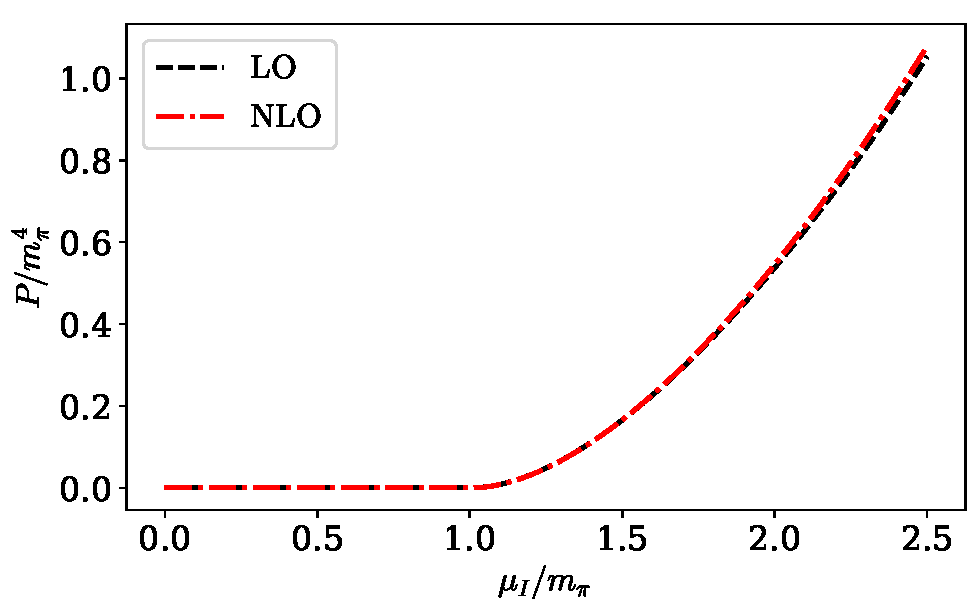
\includegraphics[width=0.7\textwidth]{figurer/numerics/pressure.pdf}
    \caption{The NLO and LO result for the pressure, as a function of $\mu_I$.}
    \label{fig:pressure}
\end{figure}

Likewise, the total isospin is proportional to volume, which means that the isospin density is
\begin{equation}
    n_I = \frac{Q_I}{V} = - \frac{1}{V} \left(\diffp{F}{\mu_I}\right)_{T, V}
    = - \diffp{\Ef}{\mu_I}.
\end{equation}
Using \cref{NLO free energy}, this equals
\begin{align}
    \nonumber
    n_I & = 
    f^2 \mu_I \sin^2 \alpha
    - \diffp{\Ef_\mathrm{fin}}{\mu_I} \\
    & + \frac{1}{(4 \pi)^2}
    \left[
            \left(2\bar l_4+\ln\frac{M^2}{m_3^2}\right)\bar m^2 \mu_I \cos\alpha \sin^2 \alpha
            +\frac{1}{3}\left(2\bar l_1 + 4 \bar l_2 + 3\ln\frac{M^2}{m_3^2}\right)\mu_I^3 \sin^4 \alpha
    \right]
\end{align}
The isospin density, as a function of $\mu_I$, is shown in \autoref{fig:isospin_density}.
\begin{figure}[h]
    \centering
    \vspace{-0.2cm}
    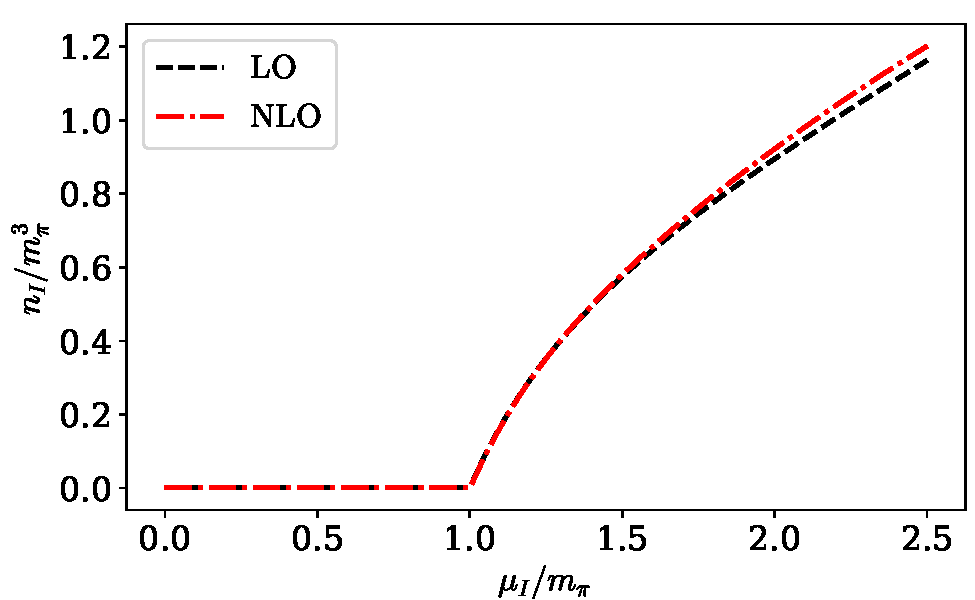
\includegraphics[width=0.7\textwidth]{figurer/numerics/isospin_density.pdf}
    \caption{The NLO and LO result for the isospin density, as a function of $\mu_I$.}
    \label{fig:isospin_density}
\end{figure}

From \cref{thermodynamic free energy} we get the energy density, $u = U/V$, at $T = 0$ is given by
\begin{equation}
    u(\mu_I) = -P(\mu_I) + \mu_I n_I(\mu_I),
\end{equation}
where we again have normalized so that $u(\mu_I = 0) = 0$.
Now that we have both the dependence of pressure and energy density on the isospin chemical potential, we can trace out the line in the pressure-energy density plane, parametrized by $\mu_I$.
This is the equation of state of the system, and is shown in \autoref{fig:equation of state}.


\begin{figure}[h]
    \centering
    \vspace{-0.2cm}
    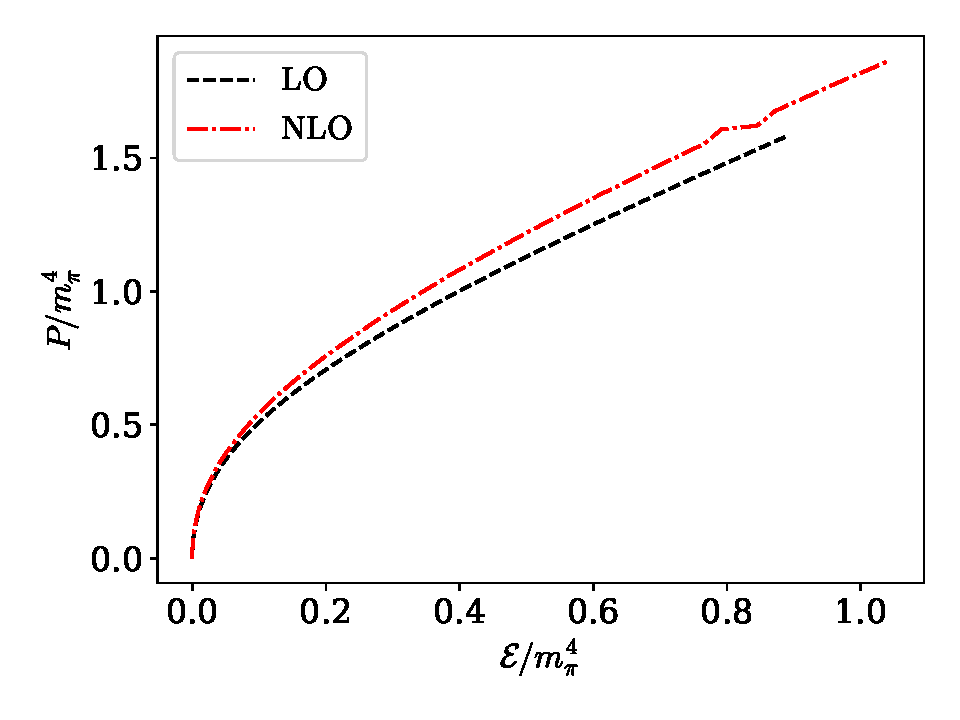
\includegraphics[width=0.7\textwidth]{figurer/numerics/energy_density.pdf}
    \caption{The leading and next-to-leading order equation of state. Both the pressure and energy density are given in units of $m_\pi^4$.}
    \label{fig:equation of state}
\end{figure}

\FloatBarrier

